\documentclass[aspectratio=169,10pt]{beamer}
\usetheme{default}
\usecolortheme{dove}
\setbeamertemplate{navigation symbols}{}
\setbeamertemplate{footline}[frame number]
\setbeamerfont{frametitle}{series=\bfseries}
\usepackage[utf8]{inputenc}
\usepackage[T1]{fontenc}
\usepackage{lmodern}
\usepackage{booktabs}
\usepackage{array}
\usepackage{graphicx}
\usepackage{xcolor}
\definecolor{good}{HTML}{0C7A0C}
\definecolor{bad}{HTML}{C0392B}
\newcommand{\ok}{\textcolor{good}{\textbf{valid}}}
\newcommand{\ko}{\textcolor{bad}{\textbf{invalid}}}

\title{Bent-crystal monochromators with xrt~2.0 and OASYS2}
\subtitle{Porting, bug fixes, reruns and next steps}
\author{M. Sanchez del Rio}
\date{29th October 2026}

\begin{document}

\begin{frame}
  \titlepage
  \centering\small
  \texttt{github.com/oasys-esrf-kit/bent\_crystals\_llnl\_esrf}\\
  \texttt{github.com/oasys-esrf-kit/OASYS2-XRT}
\end{frame}

% ---------------------------------------------------------------
\begin{frame}{LNLS XRT: four sagittally focusing bent-crystal monochromators}
  \small
  \begin{tabular}{@{}llll@{}}
    \toprule
    Beamline & Source & Monochromator & Energies \\
    \midrule
    APS\_BLM  & 7 GeV BM, 0.6 T            & Si(311) Bragg (Johann) + bent Laue & 30--60 keV \\
    SSU\_BLM  & 3 GeV BM, 6.6 T            & Si(311) Bragg (Johann) + bent Laue & 35--200 keV \\
    SSU\_SBDL & 3 GeV BM, 6.6 T            & two bent Si(111) Laue (PP)         & 35--200 keV \\
    BNL\_SBDL & 3 GeV wiggler, $K=16.5$    & two bent Si(111) Laue (ML) + Pt mirror & 30--70 keV \\
    \bottomrule
  \end{tabular}

  \vspace{1em}
  \begin{itemize}
    \item One Python script per beamline (\texttt{XRT\_*.py}) scans the energy. At each energy:
      \begin{itemize}
        \item Bragg angle, crystal positions, analytic radii $R_s$ (thin lens) and $R_m$ (anticlastic)
        \item optimization of \texttt{Fcurv}, a scale factor on the sagittal bending, to focus on the sample
        \item full trace (500k rays): flux, sizes, divergences, bandwidth, focus positions
      \end{itemize}
    \item Crystal reflectivity: use an extension \texttt{BentCrys2D.py} to compute the reflectivity of bent crystals
      using the Penning--Polder (PP, Laue only) or multilamellar (ML) model
  \end{itemize}
\end{frame}

% ---------------------------------------------------------------
\begin{frame}{What was done}
  \footnotesize
  \begin{columns}[T]
    \begin{column}{0.5\textwidth}
      \textbf{Software}
      \begin{itemize}
        \item OASYS1-XRT ported to \textbf{OASYS2-XRT}
          (\url{https://github.com/oasys-esrf-kit/OASYS2-XRT})
        \item New widgets: Bent Crystal 2D (bent Laue/Bragg Si), Bending Magnet,
          Wiggler, Johann Cylinder crystal
        \item \texttt{BentCrys2D.py} adapted to xrt~2.0 (no patched \texttt{oes\_base.py} needed)
        \item Bragg angle from xrt instead of optlnls ($\le 1.4~\mu$rad difference)
      \end{itemize}
    \end{column}
    \begin{column}{0.5\textwidth}
      \textbf{Simulations}
      \begin{itemize}
        \item All scripts run with xrt~2.0, full energy scans
        \item One OASYS2 workspace per beamline at a single energy
          (\texttt{oasys\_*/}, with \texttt{INFO.md})
        \item Internal reflectivity checked against XOPPY \texttt{diff\_pat}
        \item Two bugs found and fixed, all scans rerun
        \item Repository \url{https://github.com/oasys-esrf-kit/bent_crystals_llnl_esrf} with
          code, runs, READMEs and slides
      \end{itemize}
    \end{column}
  \end{columns}

  \vspace{0.2em}
  \centering
  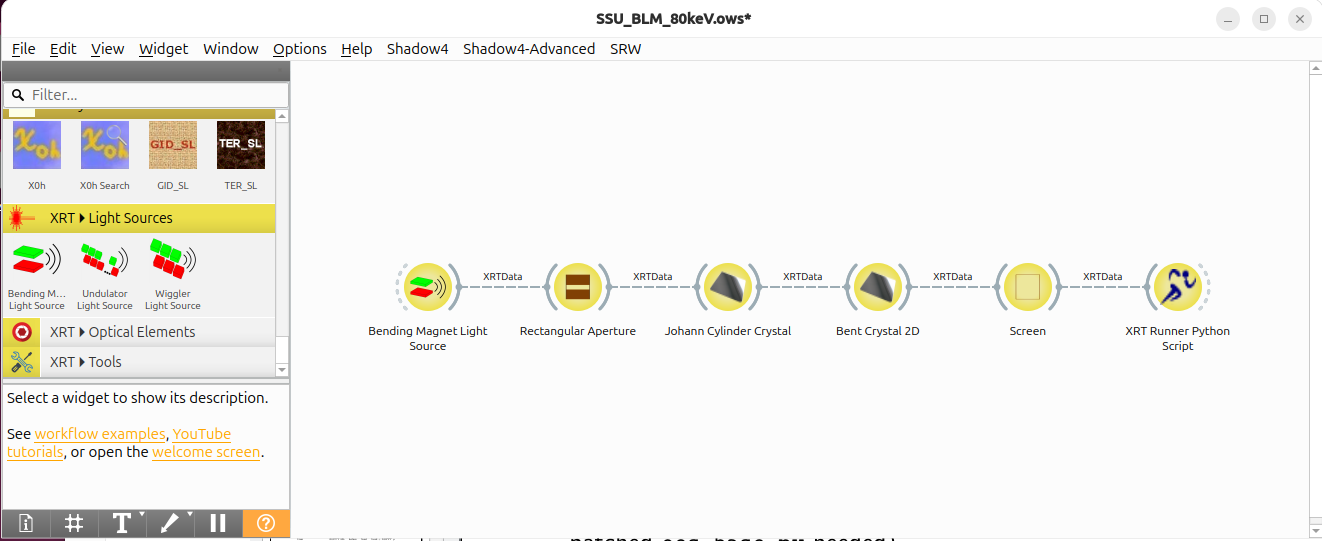
\includegraphics[width=0.9\textwidth,trim={340 175 70 205},clip]{figures/oasys_xrt.png}\\
  \scriptsize OASYS2 workspace for SSU\_BLM at 80 keV (\texttt{oasys\_SSU\_BLM/SSU\_BLM\_80keV.ows})
\end{frame}

% ---------------------------------------------------------------
\begin{frame}{How the bent-crystal model works}
  \small
  \begin{itemize}
    \item \textbf{Direction:} each ray is diffracted like a grating (surface component of
      $\mathbf{k}$ changes by the surface component of $\mathbf{H}$), using the local
      plane and surface normals of the bent crystal. Focusing comes from $R_m$ and
      $R_s\cdot$\texttt{Fcurv}.
    \item \textbf{No penetration:} rays diffract and leave at the entrance surface.
      The thickness enters only the reflectivity (no Borrmann fan, $\sim$0.1 mm for 1 mm Si at 35 keV).
    \item \textbf{Reflectivity, per ray:}
      \begin{itemize}
        \item local deviation from the Bragg condition, asymmetry from the actual directions
        \item strain gradient from the bending moments and the anisotropic compliance tensor
        \item \textbf{PP} (Laue): integration of the deviation between entrance and exit faces
        \item \textbf{ML}: lamellae summed incoherently, weighted by transmission and absorption
          (from \texttt{crystal3.f90}, as in XOPPY)
      \end{itemize}
    \item \textbf{Depth reference:} the Bragg-condition point is at the crystal
      \emph{mid-plane}; \texttt{PP\_center\_fraction} is stored but ignored.
      XOPPY uses the entrance surface. This matters later.
  \end{itemize}
\end{frame}

% ---------------------------------------------------------------
\begin{frame}{Bug 1: local beam passed downstream of the 10 m mask}
  \small
  \begin{itemize}
    \item \texttt{propagate()} and \texttt{expose()} return the beam in the
      \emph{local} frame ($y=0$). The scripts passed it to the next element as if it were global.
    \item Effect: all optics sat \textbf{10 m farther from the source}. The
      \texttt{Fcurv} optimization compensated, which is why \texttt{Fcurv} was 1.05--1.20 everywhere.
    \item Fix: pass the global beam (\texttt{beamSource}); the mask has already flagged the lost rays.
  \end{itemize}

  \vspace{0.5em}
  \centering
  SSU\_BLM at 80 keV, beam at the 56 m screen:\\[0.3em]
  \begin{tabular}{@{}lcccc@{}}
    \toprule
    Beam into Bragg & \texttt{Fcurv} & $x$ FWHM & horizontal focus & $z$ FWHM \\
    \midrule
    local (script)        & 1.1175 & 28 $\mu$m  & 56.00 m & 4.0 mm \\
    local (script)        & 1.0    & 374 $\mu$m & 52.25 m & 5.1 mm \\
    \textbf{global (correct)} & \textbf{1.0} & \textbf{40 $\mu$m} & \textbf{56.00 m} & \textbf{2.9 mm} \\
    \bottomrule
  \end{tabular}

  \vspace{0.5em}
  \raggedright
  The OASYS2-XRT Runner always used the global beam: the workspaces were correct.
\end{frame}

% ---------------------------------------------------------------
\begin{frame}{Bug 2: multilamellar (ML) reflectivity}
  \small
  Three bugs in \texttt{bentSi\_Crys.get\_amplitude}, fixed by comparison with \texttt{crystal3.f90}:
  \begin{enumerate}
    \item Laue: transmission of the lamellae in front never updated
      (\texttt{tsmall\_old}) $\Rightarrow$ $R>1$, capped at 1
    \item Lamella step refined $\times 4$; ML is incoherent, so it does not converge.
      Now $\Delta y = \pi/2$ (Laue), 2 (Bragg)
    \item xrt returns the complex conjugates of $\chi_0,\chi_H,\chi_{\bar H}$
      $\Rightarrow$ absorption acted as gain; thick Bragg crystals reflected $R\approx1$ over 330 $\mu$rad
  \end{enumerate}

  \vspace{0.3em}
  \centering
  Integrated $s$-reflectivity at 80 keV ($\mu$rad), Si(311):\\[0.3em]
  \begin{tabular}{@{}lcccc@{}}
    \toprule
    Case & XOPPY ML & before & fixed & fixed + XOPPY $\mu$ \\
    \midrule
    Laue, SSU\_BLM radii       & 34.02 & 48.77 & 30.42 & 34.04 \\
    Laue, low $R$              & 62.85 & 60.12 & 56.35 & 63.17 \\
    Bragg, SSU\_BLM            & 67.45 & 315   & 17.1  & 71.4 \\
    \bottomrule
  \end{tabular}

  \vspace{0.3em}
  \raggedright
  Remaining difference = \textbf{absorption coefficient}: xrt total $\mu = 0.521$ cm$^{-1}$
  vs XOPPY photoelectric $0.118$ cm$^{-1}$ (Si, 80 keV). Matters $\times 4$ for thick Bragg crystals.
\end{frame}

% ---------------------------------------------------------------
\begin{frame}{Laue rocking curve: internal code vs XOPPY (after the ML fixes)}
  \centering
  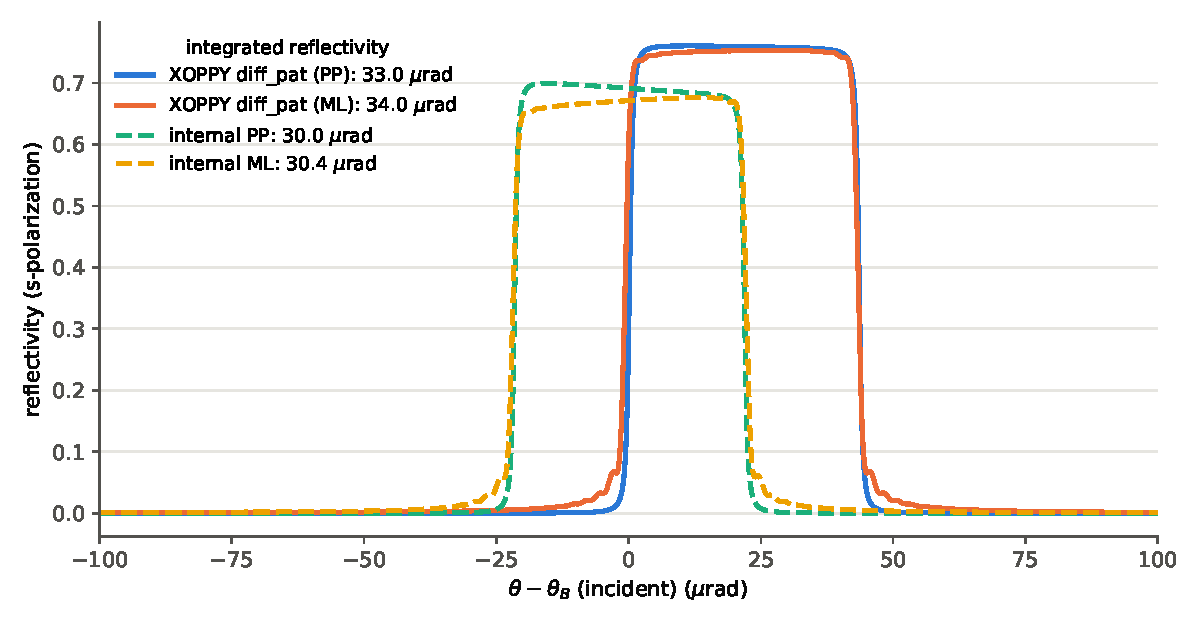
\includegraphics[width=0.70\textwidth]{figures/laue_xoppy.pdf}

  \small
  \raggedright
  SSU\_BLM Laue crystal: Si(311), 80 keV, asymmetry 20.98$^\circ$, $t = 1$ mm,
  $R_s = 1217.6$ mm, $R_m = -76039$ mm (\texttt{XOPPY/comparison\_SSU\_BLM.py}).
  \begin{itemize}
    \item Internal PP and ML now agree (PP/ML = 0.988; XOPPY 0.969), about 11\% below XOPPY
      (absorption: xrt uses the total $\mu$, possibly including Compton)
    \item The internal profiles are centred on the crystal mid-plane, XOPPY's start at the
      entrance surface: shift of half the width ($\sim$22 $\mu$rad), same integral
  \end{itemize}
\end{frame}

% ---------------------------------------------------------------
\begin{frame}{Reruns: flux at the sample}
  \begin{columns}[T]
    \begin{column}{0.56\textwidth}
      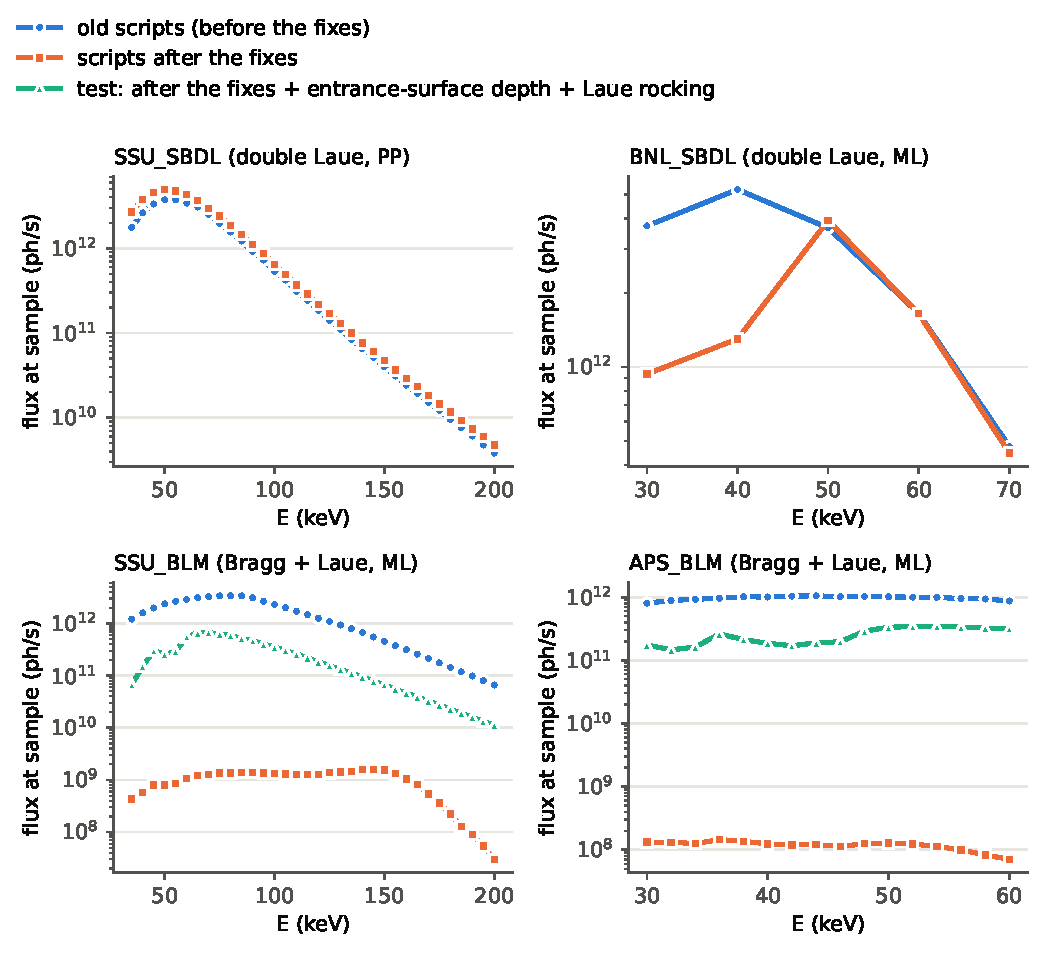
\includegraphics[height=0.83\textheight]{figures/flux.pdf}
    \end{column}
    \begin{column}{0.44\textwidth}
      \scriptsize
      \textbf{The three curves}
      \begin{itemize}
        \item \textcolor[HTML]{2a78d6}{\textbf{blue}}: old runs, with both bugs
        \item \textcolor[HTML]{eb6834}{\textbf{orange}}: the scripts with the two fixes,
          otherwise unchanged
        \item \textcolor[HTML]{1baf7a}{\textbf{green}} (Bragg+Laue only): orange + two changes
          \emph{not yet in the scripts}: (1) depth reference at the entrance surface (as XOPPY);
          (2) at each energy, the Laue pitch is scanned ($-60\ldots+160$ $\mu$rad, 5 $\mu$rad steps)
          and set to the offset of maximum intensity after the Laue crystal; the script then
          runs normally at that pitch
      \end{itemize}
      \textbf{Valid / invalid} is not about the flux level
      \begin{itemize}
        \item \ok: the simulated monochromator works (crystals aligned, focus found); the
          numbers can be quoted. SSU\_SBDL $\times$1.2--1.5, BNL\_SBDL $\times$0.25--1.07
        \item \ko\ (orange Bragg+Laue curves): in the model the Laue crystal, set at the
          nominal angle, misses the band reflected by the Bragg crystal. Only
          $10^{-4}$--$10^{-3}$ passes; sizes, bandwidth and \texttt{Fcurv} come from a few
          rays. An alignment artefact, not a property of the beamline
      \end{itemize}
    \end{column}
  \end{columns}
\end{frame}

% ---------------------------------------------------------------
\begin{frame}{SSU: double Laue (SBDL) vs Bragg + Laue (BLM)}
  \begin{columns}[T]
    \begin{column}{0.56\textwidth}
      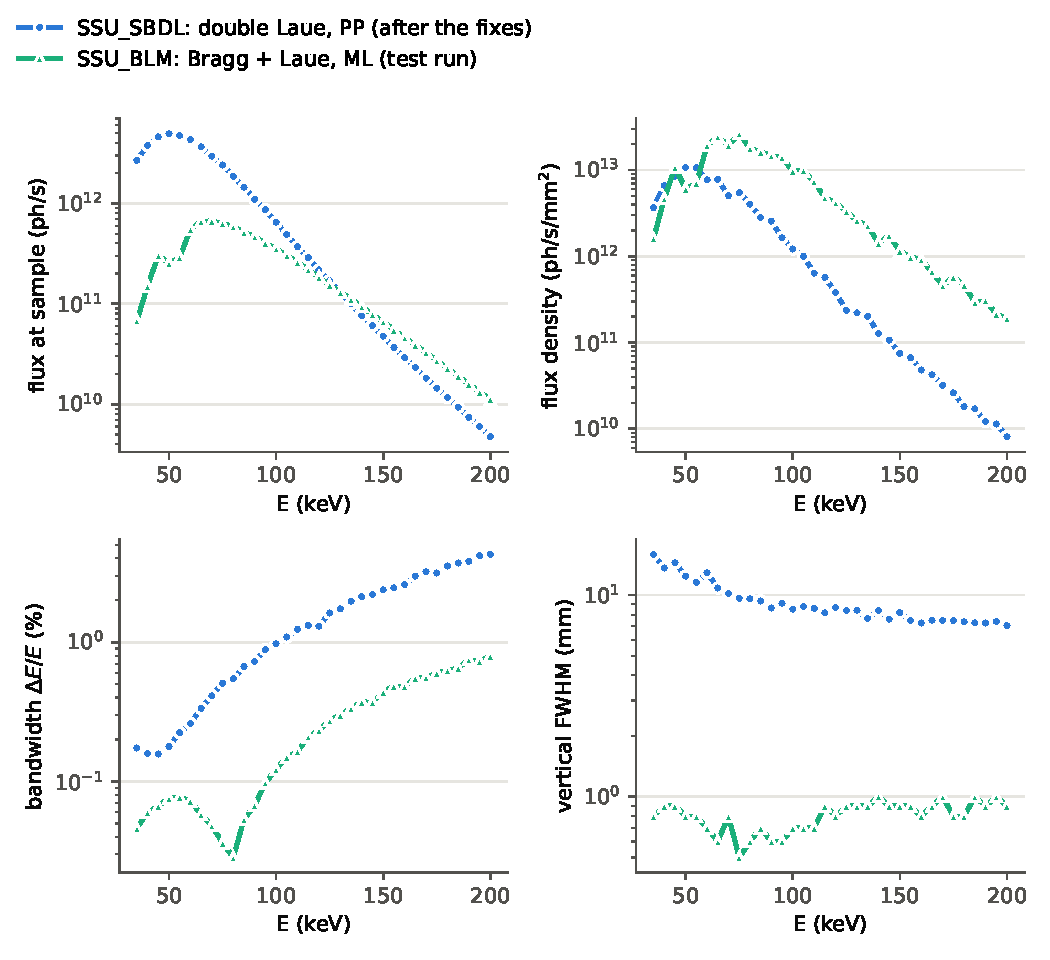
\includegraphics[height=0.83\textheight]{figures/ssu_sbdl_vs_blm.pdf}
    \end{column}
    \begin{column}{0.44\textwidth}
      \scriptsize
      Same source (3 GeV BM, 6.6 T) and same sample screen (56 m).
      \begin{itemize}
        \item \textbf{Flux:} SBDL is higher up to 130 keV ($\times$14--40 at 35--55 keV,
          $\times$3 at 80 keV); BLM is higher above 130 keV ($\times$2.4 at 200 keV)
        \item \textbf{Bandwidth:} BLM is 2--20$\times$ narrower
          ($\Delta E/E$ 0.03--0.8\% vs 0.16--4.3\%), which accounts for much of the flux
          difference
        \item \textbf{Vertical size:} BLM 0.5--1 mm (the Johann Bragg crystal focuses
          vertically), SBDL 7--16 mm (no vertical focusing)
        \item \textbf{Flux density:} so BLM wins from 60 keV on, by $\times$2.5--25
        \item \textbf{Horizontal FWHM:} similar, 34--84 $\mu$m (SBDL) and 26--60 $\mu$m (BLM)
      \end{itemize}
      \textbf{Caveats}
      \begin{itemize}
        \item SSU\_BLM is the \emph{test run} (entrance-surface depth + Laue rocking),
          not the script. It depends on the open decisions, in particular the absorption
          coefficient (up to $\times$4 on the Bragg reflectivity)
        \item SBDL uses PP for its Laue crystals, BLM uses ML (they agree within about 1\%)
      \end{itemize}
    \end{column}
  \end{columns}
\end{frame}

% ---------------------------------------------------------------
\begin{frame}{Why SSU\_BLM wins at high energy (XOPPY)}
  \begin{columns}[T]
    \begin{column}{0.56\textwidth}
      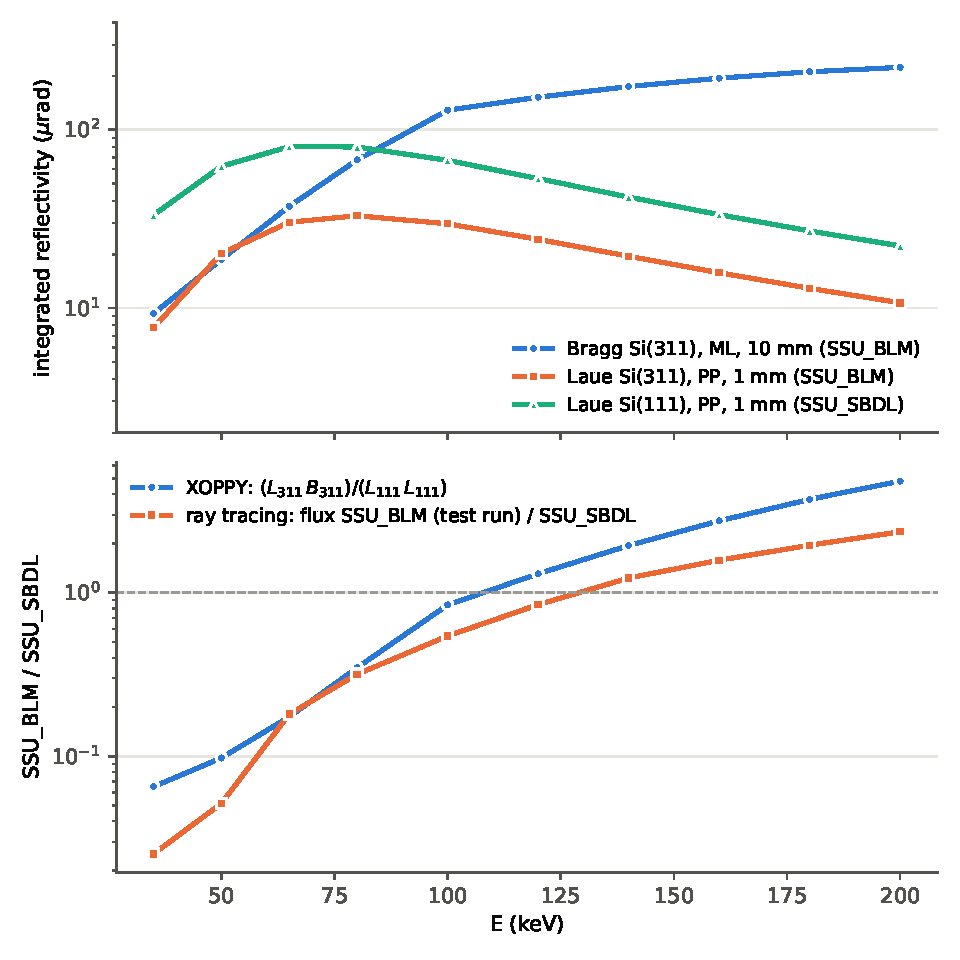
\includegraphics[height=0.83\textheight]{figures/integrated_ssu.pdf}
    \end{column}
    \begin{column}{0.44\textwidth}
      \scriptsize
      XOPPY script \texttt{XOPPY/integrated\_SSU.py}.
      \begin{itemize}
        \item \textbf{Laue, 1 mm:} peak reflectivity falls from $\sim$0.9 (65 keV) to
          0.08--0.09 (200 keV); the integrated reflectivity falls above 65--80 keV
        \item \textbf{Bragg, 10 mm bent:} peak stays $\approx$1 and the integrated
          reflectivity grows from 9 to 224 $\mu$rad
        \item So SSU\_SBDL pays the Laue loss twice, SSU\_BLM once
        \item \textbf{Figure of merit} $(L\,B)/(L\,L)$: crosses 1 at $\sim$110 keV; the
          ray tracing crosses at $\sim$130 keV, within a factor $\sim$2 everywhere
      \end{itemize}
      \textbf{Caveats}
      \begin{itemize}
        \item The product ignores how the two curves overlap for each ray
        \item XOPPY uses the photoelectric $\mu$; the ray tracing uses xrt's total $\mu$,
          which lowers the Bragg reflectivity ($\times$0.25 at 80 keV)
        \item The large SSU\_SBDL bandwidth is an energy--angle spread over the beam
          (0.66 mrad $\times\cot\theta_B$), not throughput: at 200 keV only 0.05\% of
          its 4.3\% band gets through on average (SSU\_BLM: 0.6\% of 0.8\%)
      \end{itemize}
    \end{column}
  \end{columns}
\end{frame}

% ---------------------------------------------------------------
\begin{frame}{Reruns: \texttt{Fcurv} is now $\approx 1$}
  \centering
  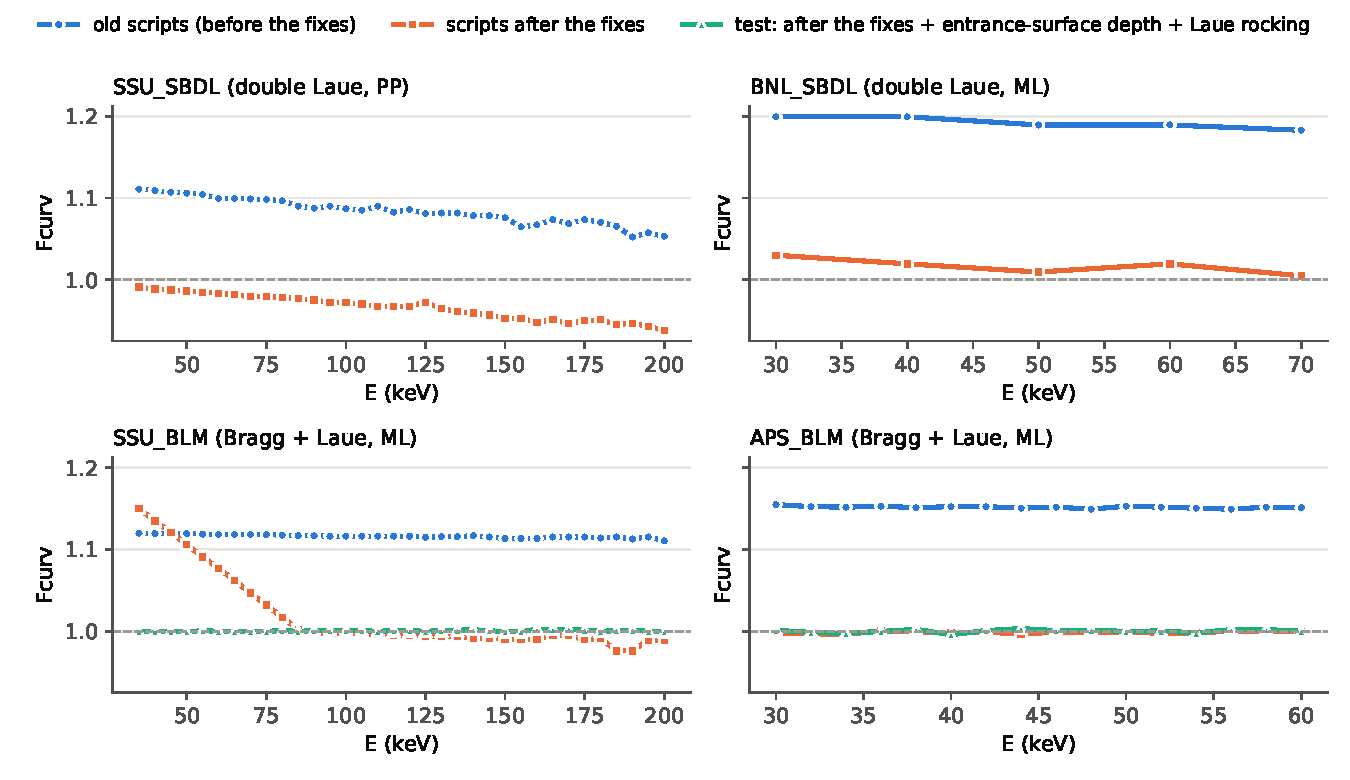
\includegraphics[width=0.82\textwidth]{figures/fcurv.pdf}

  \small
  \raggedright
  With the correct geometry the analytic radii focus on the sample
  (SSU\_SBDL 0.94--0.99, BNL\_SBDL 1.005--1.03, test runs 0.996--1.003).
  SSU\_BLM after the fixes: the search fails at low energy (no flux).
\end{frame}

% ---------------------------------------------------------------
\begin{frame}{Bragg + Laue: the reflection windows no longer overlap}
  \small
  \begin{columns}[T]
    \begin{column}{0.5\textwidth}
      \textbf{Diagnosis}
      \begin{itemize}
        \item Before the ML fix the Bragg crystal reflected over $\sim$330 $\mu$rad:
          any Laue alignment worked
        \item Now its window is narrow, and the mid-plane depth reference shifts it by
          $\sim$160 $\mu$rad in the 10 mm crystal
        \item The scripts never rock the Laue crystal
        \item Double Laue is weakly sensitive: $-20\%$ (SSU\_SBDL), $+4\%$ (BNL\_SBDL)
      \end{itemize}
    \end{column}
    \begin{column}{0.5\textwidth}
      \textbf{Test runs} (\texttt{test\_fc0\_rock/})
      \begin{itemize}
        \item \texttt{PP\_center\_fraction}$=0$ (entrance surface): profiles match
          XOPPY within 0.1 $\mu$rad
        \item Before each energy: Laue pitch scanned $-60\ldots+160$ $\mu$rad (5 $\mu$rad
          steps, 100k rays) and set to the maximum of the intensity after the Laue crystal;
          Bragg crystal untouched
        \item SSU\_BLM: best offset 0 $\to$ +120 $\mu$rad with energy, gain up to $\times$30;
          APS\_BLM: +5 to +30 $\mu$rad
        \item \texttt{Fcurv} $\approx$ 1, focus on the screen, $x$ FWHM 26--60 $\mu$m (SSU\_BLM),
          vertical 0.5--1 mm
        \item Flux 0.06--0.21$\times$ (SSU\_BLM), 0.16--0.36$\times$ (APS\_BLM) the old values,
          mostly due to $\mu$
      \end{itemize}
    \end{column}
  \end{columns}
\end{frame}

% ---------------------------------------------------------------
\begin{frame}{Summary of results after the fixes}
  \small
  \centering
  \footnotesize
  \begin{tabular}{@{}lllllc@{}}
    \toprule
    & Peak flux (ph/s) & $x$ size ($\mu$m) & $z$ size & \texttt{Fcurv} & Status \\
    \midrule
    SSU\_SBDL & $4.95\times10^{12}$ at 50 keV & 34--84   & 7--16 mm (no focusing) & 0.94--0.99  & \ok \\
    BNL\_SBDL & $3.92\times10^{12}$ at 50 keV & 404--463 & 0.11--0.13 mm          & 1.005--1.03 & \ok \\
    SSU\_BLM  & $6.7\times10^{11}$ at 70 keV  & 26--60   & 0.5--1.0 mm            & 0.999--1.002 & test run \\
    APS\_BLM  & $3.5\times10^{11}$ at 54 keV  & 167--234 & 0.45--1.15 mm          & 0.996--1.003 & test run \\
    \bottomrule
  \end{tabular}

  \vspace{1em}
  \small\raggedright
  \begin{itemize}
    \item The old results (\texttt{run\_XRT\_*/}) are superseded: wrong geometry for all four
      beamlines, wrong ML flux
    \item OASYS workspaces rerun with the fixed code: they agree with the scripts (the
      Bragg+Laue ones fail the same way)
  \end{itemize}
\end{frame}

% ---------------------------------------------------------------
\begin{frame}{Next steps}
  \small
  \textbf{Decisions}
  \begin{enumerate}
    \item \textbf{Depth reference:} implement \texttt{PP\_center\_fraction} in
      \texttt{BentCrys2D.py} and OASYS2-XRT; use 0 (entrance surface, as XOPPY) in the
      scripts, the widget default and the \texttt{.ows} files?
    \item \textbf{Second-crystal alignment:} add a per-energy Laue rocking scan to
      \texttt{XRT\_SSU\_BLM.py}, \texttt{XRT\_SSU\_BLM\_PP.py}, \texttt{XRT\_APS\_BLM.py}?
    \item \textbf{Absorption coefficient:} xrt total $\mu$ (now) or photoelectric
      (XOPPY)? $\times$4 on the Bragg integrated reflectivity.
  \end{enumerate}

  \textbf{Open questions and work}
  \begin{enumerate}\setcounter{enumi}{3}
    \item BNL\_SBDL: understand the drop to 0.25$\times$ at 30--40 keV
    \item Rerun the Bragg+Laue beamlines (and the double-Laue ones if the depth reference changes)
    \item Longer term: compare with xrt~1.x results; consider penetration (Borrmann fan)
      for the 25--60 $\mu$m foci
  \end{enumerate}
\end{frame}

% ===============================================================
\begin{frame}
  \centering
  \Large\textbf{New project: Laue and bent crystals in SHADOW4}\\[1em]
  \normalsize Plan
\end{frame}

% ---------------------------------------------------------------
\begin{frame}{Motivation and starting point}
  \small
  \textbf{Why:} SHADOW4 is the native ray tracer of OASYS2, with Jones-calculus polarization,
  but it cannot trace any of the four beamlines above: it has no Laue crystals and no bent-crystal
  reflectivities.

  \vspace{0.5em}
  \begin{tabular}{@{}>{\raggedright\arraybackslash}p{0.3\textwidth}>{\raggedright\arraybackslash}p{0.64\textwidth}@{}}
    \toprule
    Component & Status \\
    \midrule
    \texttt{S4Crystal} (SHADOW4) & Perfect crystals, Bragg only; plane, conic, toroid, mesh surfaces \\
    \texttt{S4MosaicCrystal} & Separate family of crystal classes: template for a new one \\
    crystalpy & Perfect-crystal amplitudes (Zachariasen, Guigay) for \texttt{BraggDiffraction},
      \texttt{LaueDiffraction}, \texttt{LaueTransmission}; susceptibilities from xraylib,
      DABAX or the SHADOW preprocessors \\
    \texttt{bentSi\_Crys.get\_amplitude} & PP and ML bent-crystal reflectivity per ray, now
      checked against XOPPY, but tied to xrt objects \\
	  XOPPY CRYSTAL (\texttt{diff\_pat}) & Perfect, PP, ML, Bragg and Laue \\
	  XOPPY CRYSTALPY (\texttt{crystalpy}) & Perfect Zachariasen, Guigay, Bragg and Laue \\
    \bottomrule
  \end{tabular}

  \vspace{0.5em}
  \textbf{Lessons from the xrt work to carry over:} check the sign convention of the
  susceptibilities, use the entrance-surface depth reference, validate every model against XOPPY
  before tracing a beamline.
\end{frame}

% ---------------------------------------------------------------
\begin{frame}{Steps i and ii: bent reflectivities, and bent Bragg in \texttt{S4Crystal}}
  \small
  \textbf{i) PP and ML reflectivities on a crystalpy setup}
  \begin{itemize}
    \item Extract the physics of \texttt{bentSi\_Crys.get\_amplitude} into a standalone module,
      independent of xrt: inputs are the per-ray energy, $\hat k_\mathrm{in}$, $\hat k_\mathrm{out}$,
      local Bragg-plane and surface normals, thickness, $R_m$, $R_s$, compliance tensor, model
      (PP, ML)
    \item Take $d$, $\chi_0$, $\chi_H$, $\chi_{\bar H}$ from a crystalpy \texttt{DiffractionSetup}
      (xraylib or DABAX); \textbf{verify their sign convention} (the xrt ones had to be conjugated)
    \item Implement \texttt{PP\_center\_fraction} (depth reference), default entrance surface
    \item Validate: rocking curves and integrated reflectivities vs XOPPY \texttt{diff\_pat}
      (SSU\_BLM and SSU\_SBDL crystals, 35--200 keV) and vs the xrt implementation
  \end{itemize}

  \textbf{ii) Bent Bragg (ML only) in \texttt{S4Crystal}}
  \begin{itemize}
    \item New option for the reflectivity model: perfect (crystalpy, as now) or bent ML
    \item Directions stay as now (crystalpy, local normal of the surface); only $r_\sigma$, $r_\pi$
      change: $\sqrt{R}$, no phase (incoherent model)
    \item Bending radii given explicitly (they need not equal the surface curvature, cf.\
      \texttt{Fcurv}); cylinder/toroid surfaces for the shape
    \item Test case: SSU\_BLM Bragg crystal (Si(311), 10 mm, $R_m = 647.7$ m); compare with XOPPY
      ML and with the xrt Johann cylinder
  \end{itemize}
\end{frame}

% ---------------------------------------------------------------
\begin{frame}{Steps iii and iv: \texttt{S4LaueCrystal} and penetration}
  \small
  \textbf{iii) New \texttt{S4LaueCrystal}} (family of classes for plane, cylinder, toroid, as for mosaic crystals)
  \begin{itemize}
    \item Laue alignment and geometry: beam enters the front face, diffracted beam leaves the back face
    \item Reflectivity models:
      \begin{itemize}
        \item perfect crystal: crystalpy \texttt{LaueDiffraction} (Zachariasen/Guigay), as SHADOW3
          did for Laue crystals
        \item bent crystal: PP and ML from step i
      \end{itemize}
    \item Validate: vs XOPPY (perfect, PP, ML), vs SHADOW3 for perfect Laue, and full beamlines
      SSU\_SBDL and SSU\_BLM vs xrt
  \end{itemize}

  \textbf{iv) Penetration in \texttt{S4LaueCrystal}}
  \begin{itemize}
    \item Today (xrt with the \texttt{BentCrys2D} extension) rays diffract and leave at the entrance surface. The real beam
      leaves from the back face, spread over the Borrmann fan ($2t\tan\theta_B$ symmetric: $\sim$0.1 mm
      at 35 keV for 1 mm), comparable to the 25--60 $\mu$m foci
    \item Study: where to place the exit point? This influences the ``polychromatic focusing''
    \item Include it as an option and quantify its effect on the focal sizes (SSU\_SBDL, SSU\_BLM)
  \end{itemize}
\end{frame}

% ---------------------------------------------------------------
\begin{frame}{Plan: order, deliverables and checks}
  \footnotesize
  \centering
  \begin{tabular}{@{}clll@{}}
    \toprule
    Step & Deliverable & Check & Depends on \\
    \midrule
    i   & bent reflectivity module (PP, ML), crystalpy setup     & XOPPY \texttt{diff\_pat}, xrt & -- \\
    ii  & \texttt{S4Crystal} with bent ML Bragg                  & XOPPY ML, xrt Johann         & i \\
    iii & \texttt{S4LaueCrystal}: perfect, PP, ML                & XOPPY, SHADOW3, xrt & i \\
    iv  & penetration option in \texttt{S4LaueCrystal}           & focal sizes with/without      & iii \\
    --  & OASYS2 widgets, example workspaces                     & the four beamlines            & ii, iii \\
    \bottomrule
  \end{tabular}

  \vspace{1em}
  \small\raggedright
  \begin{itemize}
    \item The open decisions of the xrt study (depth reference, second-crystal alignment,
      absorption coefficient) apply here too and should be settled first
    \item End point: the four beamlines traced in both xrt and SHADOW4, with the same crystal
      physics, as a cross-check of both codes
  \end{itemize}
\end{frame}

\end{document}
